% ---------------------------------------------------------------------------
% LXAI @ NeurIPS 2026 -- LatinX in AI Research Workshop
% Category: FULL PAPER (up to 8 pages excluding references).
%
% CAMERA-READY VERSION, accepted. No longer double blind: it carries 'final' in
% the style options and the \author block below. To go back to an anonymous
% version (for another submission under review, say) drop 'final' and the style
% hides the authors and the 'ack' environment on its own.
%
% neurips_2025.sty is the most recent official NeurIPS style; the 2026 one is
% not out yet (the CFP link points at a 2015 page that was never updated).
%
% The three items that were missing are now in place, as given by the authors:
%   1. The emails, in the \author block below.
%   2. The 'ack' environment, just before the bibliography: there was no
%      external funding and there are no competing interests.
%   3. The repository URL, in the Limitations footnote.
% ---------------------------------------------------------------------------
\documentclass{article}

\usepackage[dblblindworkshop, final]{neurips_2025}
\workshoptitle{LatinX in AI (LXAI) Research Workshop}

% The available .sty is the 2025 one and this goes to NeurIPS 2026, the 40th
% edition. This only fixes the footer notice; if LXAI publishes a
% neurips_2026.sty, swap the package in and delete these four lines.
\makeatletter
\renewcommand{\@neuripsordinal}{40th}
\renewcommand{\@neuripsyear}{2026}
\makeatother

\usepackage[utf8]{inputenc}
\usepackage[T1]{fontenc}
\usepackage{etoolbox}

% The official NeurIPS example PDF ships VECTOR typewriter (SFTT1000, which
% cm-super provides) and Computer Modern maths. Without cm-super installed,
% cmtt under T1 falls back to Type 3 bitmaps and goes blurry on zoom. ONLY the
% monospaced family is substituted, by Latin Modern, which is vector and from
% the same design family. lmodern is NOT loaded whole: that would take out the
% Times body text and the CM maths, which are what the NeurIPS style fixes.
\renewcommand{\ttdefault}{lmtt}
\usepackage{amsmath,amssymb}
\usepackage{booktabs}
\usepackage{graphicx}
\usepackage{microtype}
\usepackage{url}
\usepackage{xcolor}
% In the camera-ready the PDF metadata IS filled in: the anonymity check
% required an empty Title and Author, and that no longer applies.
\usepackage[colorlinks=true,allcolors=blue!60!black,
            pdftitle={Your Ground Truth Is Running the Same Biased Estimator as Your Method:
                      Incorporation Bias in the Geometric Evaluation of Segmentation Pipelines},
            pdfauthor={Manuel Josue Malla Campoverde, Eduardo Tusa}]{hyperref}
\usepackage{caption}
\captionsetup{font=small,labelfont=bf}

\newcommand{\pct}[1]{$#1\,\%$}

% The checklist was numbered as "Table" in its caption but cited as "Box" in
% the text. It gets its own float type and its own counter.
\usepackage{float}
\newfloat{algbox}{tbp}{lob}
\floatname{algbox}{Box}

% The checklist was numbered as "Table" in the caption and cited as "Box" in
% the text. It gets its own float type and its own counter.


% The audit table overflowed the margin by 13.3pt. Column separation is
% tightened inside table environments only, without touching the geometry or
% the body text (shrinking text to fit content in is a formatting violation
% that the chairs do check).
\AtBeginEnvironment{table}{\setlength{\tabcolsep}{4.5pt}}

% This paper is deliberately visual: 3 figures and 4 tables in 8 pages. The
% LaTeX defaults (2 floats at the top, 3 per page, 20 % minimum text) push
% floats to the end and waste half a page, so they are relaxed. This does NOT
% shrink text or touch margins: it only changes where a float may go.
\setcounter{topnumber}{3}
\setcounter{bottomnumber}{2}
\setcounter{totalnumber}{4}
\renewcommand{\topfraction}{0.92}
\renewcommand{\bottomfraction}{0.75}
\renewcommand{\bottomfraction}{0.75}
\renewcommand{\textfraction}{0.07}
\renewcommand{\floatpagefraction}{0.75}

\title{Your Ground Truth Is Running the Same Biased Estimator as Your Method:\\
       Incorporation Bias in the Geometric Evaluation of Segmentation Pipelines}

% Names are spelled as the authors write them; inputenc utf8 is already loaded,
% so an accent can go in directly. Both institutional emails are filled in.
\author{%
  Manuel Josue Malla Campoverde \\
  Universidad T\'ecnica de Machala \\
  Machala, Ecuador \\
  \texttt{mmalla1@utmachala.edu.ec} \\
  \And
  Eduardo Tusa \\
  Universidad T\'ecnica de Machala \\
  Machala, Ecuador \\
  \texttt{etusa@utmachala.edu.ec} \\
}

\begin{document}
\maketitle

\begin{abstract}
Segmentation masks are routinely turned into physical quantities --- perimeter in centimetres,
circularity, radiomic shape features --- that are then compared against the world. The
boundary-length estimator shipped by the default stack has had a closed-form bias since 1979 and has
been provably non-convergent since 2003, and coupling such an estimator into a synthetic reference
is a known failure mode: the \emph{inverse crime}. \emph{We claim none of that.} What we report is
that its standard antidote fails here: refining the reference grid cannot separate reference from
method when the shared component has a bias floor. On our test shape binary marching squares
self-converges at order $2.79$ while its true error sits at a constant \pct{+8.20}. In a
leaf-phenotyping pipeline of our own this hid a \pct{+4.55} perimeter error behind a reported
\pct{-0.01}, and a flat-mesh extractor appeared to beat a raster baseline while being nearly three
times worse --- a \pct{+3.87} digitisation bias cancelling a \pct{-7.69} projection bias --- for
which we give the closed-form condition. Auditing the stack (scikit-image, OpenCV, PlantCV,
HistomicsTK, PyRadiomics, IBSI), most of it is silent where the feature is defined, and the remedy
it recommends is not independent either: four-direction discrete Crofton is \emph{exactly} marching
squares divided by Kulpa's constant on saddle-free masks. The failure is larger in three dimensions:
PyRadiomics returns sphericity $0.919$ for a perfect digital sphere, at every resolution. We propose
a reference-estimator rule stronger than independence alone, a three-grid screening test for the
failure, and a convergent estimator that cuts our leaf error to \pct{-0.26} at comparable cost.
\end{abstract}

% ===========================================================================
\section{Introduction}
% ===========================================================================

A large and growing body of applied machine-learning work ends by turning a predicted mask into a
number with units: leaf perimeter and lesion compactness in phenotyping, nuclear circularity in
digital pathology, \texttt{shape2D} descriptors fed to radiomics classifiers and then used to
explain them, patch edge length in remote sensing. The mask stops being a set of pixels and becomes
a measurement compared against a physical or clinical reference.

The estimator that performs that conversion is almost never questioned. Applying
marching squares at level $0.5$ to a binary mask, the default route in the mainstream libraries
we checked produces a polygon whose vertices sit at edge midpoints between an inside and an
outside pixel: exactly the naive $8$-connected chain-code estimator with weights $(1,\sqrt2)$,
whose bias has a closed form from 1979~\citep{proffitt1979} and whose correction factor for smooth
shapes dates to 1977~\citep{kulpa1977}. \citet{tajine2003} proved that \emph{no} length estimator
built on a finite number of local configurations can be multigrid-convergent, whatever weights it
uses, which covers the weighted variants~\citep{dorst1987} as well as the naive
one~\citep{coeurjolly2012,coeurjolly2004,klette2004}; convergent alternatives with proofs have been
catalogued for two decades~\citep{kovalevsky1992,sloboda1998,lachaud2007,provencal2009}.

None of this is our contribution. Our contribution is what this known bias did to a real
pipeline once it was allowed into the \emph{reference}.

We built a geometric pipeline that converts segmentation masks of a banana leaf into agronomic
parameters through constrained Delaunay triangulation and P1 finite elements, and validated it
against a synthetic leaf with analytically exact ground truth. It reported a perimeter error of
\pct{-0.01}. That number was an artefact: the generator computed its reference with the same binary
marching-squares call the pipeline used, so two implementations of one bias were measuring each
other. The true error was \pct{+4.55}.

This mechanism is known and named. In inverse problems it is the \emph{inverse
crime}~\citep{coltonkress,wirgin2004} --- ``the same (or very nearly the same) theoretical
ingredients are employed to synthesize as well as to invert data'' --- formalised as a
discretisation artefact by \citet{kaipio2007}, with relatives in diagnostic
accuracy~\citep{whiting2011}, systems neuroscience~\citep{kriegeskorte2009}, and the
code-verification hierarchy that ranks code-to-code comparison last for common-mode
error~\citep{oberkampf2010}. We claim none of it.

What we report is that the standard antidote fails here. The prescription against an inverse crime
is to generate the reference on a finer, non-nested grid, advice that presumes refinement
eventually separates the two. It does not when the shared component is a non-convergent estimator,
whose error has a floor independent of $h$~\citep{tajine2003}. Figure~\ref{fig:selfconv} measures
this: binary marching squares self-converges at observed order $2.79$ while its true error sits at
a constant \pct{+8.20}, and worse, the study ranks the estimators \emph{backwards}, flattering the
two that never converge.

\paragraph{Contributions.}
\begin{enumerate}\itemsep1pt
  \item The standard remedy for an inverse crime --- refine the reference grid --- cannot work
        when the shared component is non-convergent, and we measure the self-convergence that
        results (\S\ref{sec:case}).
  \item We quantify the damage: the coupling \emph{inverted the ranking} of two contour
        extractors, and fixing the reference alone does not undo it (\S\ref{sec:inversion}).
  \item We audit the stack --- scikit-image, OpenCV, PlantCV, HistomicsTK, PyRadiomics, IBSI ---
        show its recommended remedy is the same estimator rescaled, and carry the result to 3D
        surface area, where it is larger (\S\ref{sec:stack}).
  \item We give a reference-estimator rule stronger than independence alone, a three-grid test
        that screens for it, and a convergent estimator measured against the default
        (\S\ref{sec:fix}).
\end{enumerate}

% ===========================================================================
\section{Background: a bias with a closed form since 1979}
\label{sec:background}
% ===========================================================================

Let $\theta$ be the angle of a straight boundary segment with respect to the pixel grid
axes, folded into $[0^\circ,45^\circ]$ by symmetry. A segment of length $L$ digitises to $L\sin\theta$
diagonal steps of weight $\sqrt2$ and $L(\cos\theta-\sin\theta)$ axis-aligned steps of weight $1$,
so the naive $8$-connected chain-code estimator --- marching squares on a binary indicator ---
returns asymptotically
\begin{equation}
  \frac{L_{\text{est}}}{L_{\text{true}}} \;=\; \cos\theta + (\sqrt{2}-1)\,\sin\theta .
  \label{eq:pr}
\end{equation}
This is the metrication error of chain-encoding schemes analysed by \citet{proffitt1979}, whose
weighted correction is the standard remedy. Since $\sqrt2-1 = \tan 22.5^\circ$, \eqref{eq:pr} is a
cosine of amplitude
$\sec 22.5^\circ = 1.0824$ centred on $22.5^\circ$: the ratio is $1$ at $0^\circ$ and $45^\circ$
and peaks at \pct{+8.24} between them, and our measured sweep tracks it with an RMS deviation of
$0.074$ percentage points. Averaging \eqref{eq:pr} uniformly over orientations gives
$\tfrac{4}{\pi}(2\sqrt2-2) = 1.05479$, the classical correction factor of \citet{kulpa1977}.
Uniform is the arc-length average only where the tangent turns at a constant rate --- arc length
weights each direction by the radius of curvature --- so the constant is exact for a circle and not
for other convex curves: over ellipses of growing eccentricity the arc-length average of
\eqref{eq:pr} falls to \pct{+2.02} while the uniform value stays at \pct{+5.48}, and measurement
follows the former to $0.034$\,pp. A constant derived for one shape does not correct the others,
which is also why a circle cannot test an estimator carrying it (Box~\ref{box:test}).

Table~\ref{tab:closed} checks our measurements against these closed forms. We report the agreement
deliberately rather than as a finding: it calibrates the instrument.

\begin{table}[htbp]
\centering
\caption{Our measurements are the 1977--1979 closed forms, on a $3200^2$ grid over
$[-1.6,1.6]^2$. This calibrates the instrument; it is not a result.}
\label{tab:closed}
\small
\begin{tabular}{llrr}
\toprule
Shape & Predicted by & Closed form & Measured \\
\midrule
Circle, $r=1$                     & Kulpa \citeyearpar{kulpa1977}; \eqref{eq:pr} averaged & $+5.479\,\%$ & $+5.485\,\%$ \\
Square rotated $22.5^\circ$       & \eqref{eq:pr} at its maximum                          & $+8.24\,\%$  & $+8.307\,\%$ \\
Square rotated $0^\circ/45^\circ$ & \eqref{eq:pr} at its zeros                            & $0\,\%$      & $-0.04\,/\,-0.09\,\%$ \\
\bottomrule
\end{tabular}
\end{table}

Two properties of \eqref{eq:pr} matter for what follows, and both are counterintuitive.

\paragraph{The bias does not vanish with resolution.} It converges --- to the wrong value.
Across a $16\times$ range of grid spacings the binary estimator stays flat at \pct{+5.5} on a
circle and \pct{+7.3} on a rotated square, while a consistent estimator falls with the grid
(Fig.~\ref{fig:selfconv}b). More pixels buy nothing. This is the practical content of the \citet{tajine2003}
impossibility theorem, and it applies to any estimator reading a fixed local neighbourhood:
marching squares is a $2\times2$ lookup, \texttt{skimage.measure.perimeter} a weighted
local-configuration count, \texttt{cv2.arcLength} a walk over border-pixel centres.

\paragraph{The bias depends on how the object is rotated.} Figure~\ref{fig:orientation}
sweeps the orientation of a square and finds the error moving from \pct{0} to \pct{+8.1}
and back, tracking Eq.~\eqref{eq:pr}. Across ten rotations of the same shape at
fixed resolution, the binary estimator spreads over $8.13$\,pp while a zero-level-set
estimator spreads over $0.023$\,pp --- a factor of $347$. Any downstream analysis
that compares a shape descriptor between objects, or between images, is therefore
comparing a quantity that partly encodes the object's angle with respect to the sensor.

\begin{figure}[tb]
\centering
\begin{minipage}[t]{0.485\textwidth}
  \centering
  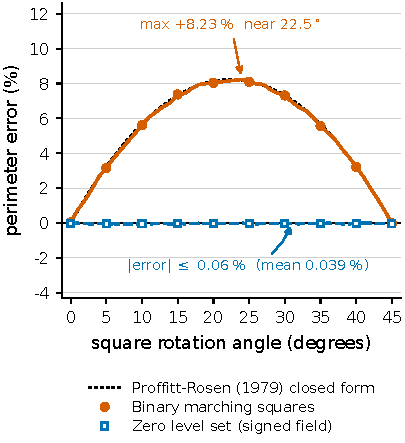
\includegraphics[width=\linewidth]{fig/fig1_orientation.pdf}
  \caption{Perimeter error of a square against its rotation, at fixed resolution. The binary
  estimator follows the 1979 closed form; the zero-level-set estimator stays at zero. The measured
  quantity partly encodes the object's angle relative to the pixel grid.}
  \label{fig:orientation}
\end{minipage}\hfill
\begin{minipage}[t]{0.485\textwidth}
  \centering
  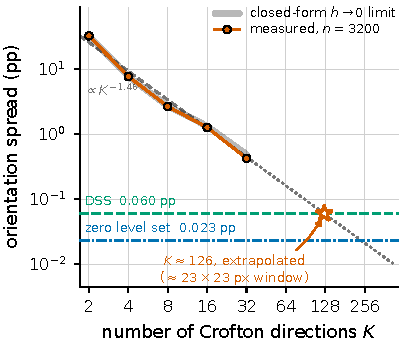
\includegraphics[width=\linewidth]{fig/fig7_crofton.pdf}
  \caption{More directions help and never suffice. Orientation spread against the number of
  Crofton directions $K$, with the limit each $K$ stalls at. Matching a convergent estimator needs
  a neighbourhood that is no longer local.}
  \label{fig:crofton}
\end{minipage}
\end{figure}

\begin{figure}[tb]
\centering
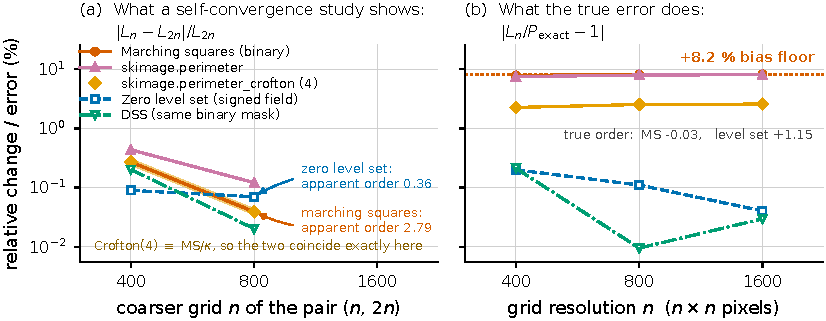
\includegraphics[width=\textwidth]{fig/fig5_selfconv.pdf}
\caption{Why refining the reference grid cannot expose the problem. Square at $22.5^\circ$,
$n = 400, 800, 1600$. \textbf{(a)} What a self-convergence study sees --- successive differences,
the only thing measurable without exact truth. Every estimator looks convergent and the ranking is
\emph{backwards}. \textbf{(b)} The true errors reveal persistent bias floors for marching squares and Crofton, while the zero-level-set estimator continues to decrease over the tested resolutions. Crofton coincides with marching squares in (a) because it is that estimator divided
by a constant, which cancels in a relative difference.}
\label{fig:selfconv}
\end{figure}

% ===========================================================================
\section{The stack ships it anyway}
\label{sec:stack}
% ===========================================================================

If this were confined to the digital-geometry literature it would be a curiosity. Table~\ref{tab:audit}
records what the tools an applied ML practitioner reaches for do, and how they document it.\footnote{Audited 18 August 2026: for each tool, the docstring or manual entry where the
perimeter feature is defined, the rendered documentation page including gallery examples
back-referenced from it, and the source where public. scikit-image 0.25.2 and
0.26.0~\citep{vanderwalt2014}, OpenCV 4.13.0~\citep{bradski2000}, PlantCV
4.11.3~\citep{gehan2017}, HistomicsTK 1.4.0, PyRadiomics 3.0.1~\citep{vangriethuysen2017}, the
IBSI manual~\citep{ibsi2019} and standard~\citep{zwanenburg2020}, FRAGSTATS
v4~\citep{mcgarigal2023}. Issue-tracker discussion was not counted, though scikit-image issues \#3573 and \#3812 have raised
perimeter accuracy since 2018 without reaching the docstrings.}

\begin{table}[htbp]
\centering
\caption{Audit of the default stack. ``Warns?'' asks whether the documentation or source
\emph{states}, where the feature is defined, that the estimator is biased or depends on
resolution or orientation; we separate a stated caveat from a demonstration the reader must
interpret unaided. Measured columns are ours, on a $3200^2$ grid; spread is
$\max_\theta e(\theta) - \min_\theta e(\theta)$ in percentage points over ten rotations of a
square.}
\label{tab:audit}
\small
\begin{tabular}{llcrr}
\toprule
Tool / standard & Perimeter route & Warns? & Circle & Orient.\ spread \\
\midrule
\texttt{skimage.measure.perimeter}      & local configurations         & shown$^\dagger$   & $+5.44\,\%$  & $8.10$\,pp \\
\texttt{skimage.\,perimeter\_crofton}   & discrete Crofton, 4 dir.     & shown$^\dagger$   & $+0.006\,\%$ & $7.71$\,pp \\
\texttt{cv2.arcLength}                  & border-pixel chain           & no                & $+5.44\,\%$  & $8.13$\,pp \\
PlantCV \texttt{analyze.size}           & calls \texttt{cv2.arcLength} & no                & \multicolumn{2}{c}{inherits} \\
HistomicsTK morphometry                 & calls \texttt{regionprops}   & no$^\ddagger$     & \multicolumn{2}{c}{inherits} \\
PyRadiomics \texttt{shape2D\_Perimeter} & marching-squares mesh        & no$^{\S}$         & \multicolumn{2}{c}{inherits} \\
IBSI                                    & recommends marching cubes    & \textbf{yes}$^{\P}$ & \multicolumn{2}{c}{---} \\
\midrule
FRAGSTATS (landscape ecology)           & raster edge length           & \textbf{yes}      & \multicolumn{2}{c}{---} \\
\bottomrule
\end{tabular}
\vspace{3pt}
\parbox{0.97\textwidth}{\footnotesize $^\dagger$Demonstrated in a gallery example linked from the
API page, never stated (see text). $^\ddagger$Discloses the mechanism --- ``a line through the
centers of border pixels using a 4-connectivity'' --- but no direction of error.
$^{\S}$Documents the derived \texttt{Sphericity} as ``independent of scale and orientation'', an
affirmative claim of the property the measurement lacks. $^{\P}$States the bias, then prescribes
an estimator of the same class (see text).}
\end{table}

Three observations. First, \texttt{perimeter\_crofton} looks much better on smooth
boundaries --- \pct{+0.006} on a circle --- but it is still a finite local-configuration
estimator, so the impossibility theorem covers it too. Rotating a single square exposes this
immediately: its error runs from \pct{-5.18} at $0^\circ$ to \pct{+2.52} at $25^\circ$, a spread
of $7.71$\,pp against marching squares' $8.13$\,pp. The similarity is not accidental. On
any mask free of saddle configurations, \texttt{perimeter\_crofton} with four directions returns
\emph{exactly} the marching-squares length divided by the Kulpa constant
$\tfrac{4}{\pi}(2\sqrt2-2) = 1.05479$: we verified the identity on all $23\,857$ saddle-free
subsets of a $4\times4$ window with zero residual, and on our leaf mask, which contains no saddle
in $251\,937$ windows, the two agree bit for bit after rescaling. The recommended remedy is not an
independent estimator at all: it is the same functional with the $1977$ correction already applied,
near-exact on the smooth shape the constant was derived for and carrying the orientation dependence
everywhere else. Adding directions helps and does not fix it (Fig.~\ref{fig:crofton}): each $K$ stalls at an
analytically predicted non-zero limit, and at every fixed $K$ the impossibility theorem still
applies.

Second, the bias propagates into derived features silently. HistomicsTK defines circularity as
$4\pi A/P^2$; since $A$ converges and $P$ carries \pct{+5.4}, circularity of a smooth object comes
out roughly \pct{10} low, by an amount that changes as the object rotates. PyRadiomics derives
\texttt{Sphericity} and \texttt{PerimeterSurfaceRatio} from the same perimeter.

Third, and this is why we think the paper belongs at a machine-learning venue rather than a geometry
one: the chain reaches current work. A 2026 study applies PyRadiomics to segmented banana leaf masks
to characterise Fusarium wilt and black Sigatoka~\citep{sigatoka2026} --- the same crop and disease
as the pipeline of \S\ref{sec:case} --- and reports that higher values of
\texttt{original\_shape2D\_Perimeter}, \texttt{PerimeterSurfaceRatio} and
\texttt{MajorAxisLength} contributed positively to Sigatoka predictions. The model's explanation
therefore rests on features whose value depends on how the lesion happened to be oriented with
respect to the pixel grid. We single it out not because it is unusual but because it is exemplary:
careful, recent, using the reference implementation of an international standard, and inheriting a
bias that has had a closed form for forty-seven years.

Two rows deserve more care than a binary column allows, and both sharpen the picture.
\textbf{IBSI does warn}: where the morphological features are defined, the manual states that
``voxel-based representations lead to partial volume effects and over-estimation of the surface
area''~\citep{ibsi2019}. The diagnosis is exact; the prescription carries the problem forward. It
recommends marching cubes~\citep{lorensen1987} --- a fixed $2\times2\times2$ neighbourhood, so a
local estimator in precisely the sense of \citet{tajine2003} --- and calls that representation
``independent of size'', the one property such an estimator lacks; the citation attached to its
``reasonable approximation'' is \citet{stelldinger2007}, which proves the reconstruction
\emph{homeomorphic} to the object, a topological guarantee offered for a metric claim.
\textbf{scikit-image cuts the other way}: its docstrings say nothing, but the rendered API page of
both perimeter functions links a gallery example that rotates a square and a disk through
$90^\circ$ and plots four estimators against ground truth --- shipped since 2020, and essentially
our Figure~\ref{fig:orientation}. What it does not do is say what it shows: one sentence of prose,
no conclusion, and a remark on grid size pointing towards more resolution, which smooths the curve
and leaves the bias.

\paragraph{The same failure in three dimensions.} Clinical radiomics measures surface area by
marching cubes on the binary mask; Figure~\ref{fig:surf3d} repeats the experiment there.
Equation~\eqref{eq:pr} generalises: the half-space ratio is again exactly $1$ at the three cubic
symmetry directions and averages to $\bar f_{3\mathrm D} = 1.08827$ over $S^2$ against Kulpa's
$1.05479$, measured rather than derived. Because voxel-counted volume is convergent, the bias
passes into sphericity. One qualification: on smooth bodies it is close to a constant offset, and
the orientation dependence returns only for faceted objects.

Read together with FRAGSTATS, which names mechanism and direction but never orientation, these
point somewhere more specific than a failure of transfer. The knowledge did reach the stack; what
is missing at every step is the criterion. Nothing in this chain asks whether the estimator
converges.

% ===========================================================================
\section{A pipeline that fooled itself}
\label{sec:case}
% ===========================================================================

\paragraph{Setting.} We study a pipeline that turns three binary masks (blade, lesions, midrib)
into agronomic parameters via a constrained Delaunay mesh~\citep{shewchuk1996} and P1
finite-element operators. It runs at three levels so causes can be separated: \textbf{A}, raster
only (Crofton perimeter); \textbf{B}, flat mesh; \textbf{C}, mesh lifted onto a cylinder to undo
the leaf's curl.

Validation uses a synthetic leaf whose ground truth is analytic: the blade is embedded by an
isometry, so intrinsic lengths and areas are known in closed form. This is the standard and, we
still believe, correct way to validate such a pipeline. It is also what created the problem.

\paragraph{The coupling.} The generator needed a perimeter for the blade outline, a
piecewise-analytic curve with tears. Rather than integrate arc length over the boundary
description, it rasterised the blade and ran marching squares on the binary indicator --- the same
call, in the same library, the meshing module used to turn a mask into a polygon.

\paragraph{What it hid.} The biased reference put the intrinsic perimeter at $778.17$\,cm and level
C measured $778.06$\,cm, so the reported \pct{-0.014} became the project's headline accuracy number.
A consistent reference gives $744.23$\,cm intrinsic and $686.98$\,cm projected: the projection
factor is \pct{-7.69} and level C's true error \pct{+4.55}. The two references differ by
\pct{+4.56} --- the estimator's bias on this shape --- and the method carried \pct{+4.55} of it. The
agreement was not accuracy; it was the bias cancelling against itself.

\paragraph{Why the usual safeguard failed.} The project had a refinement study; it passed, and it
could not have failed. Refining sixteenfold, from $h=0.4$ to $0.025$\,cm, the binary estimator
settles \pct{+4.72} above the consistent one and stays. A statistical double-dip inflates an
estimate; this one inflates it \emph{and} disarms the diagnostic that would catch it.

% ===========================================================================
\subsection{The ranking inversion}
\label{sec:inversion}
% ===========================================================================

The inflated accuracy is bounded; the consequential damage is that the biased reference reverses the comparison between methods.

The original project exposed a single ground-truth perimeter, $778.17$\,cm, and divided all three
levels by it; the intrinsic/projected distinction did not exist until the estimator was replaced.
Table~\ref{tab:inversion} reproduces that reading in column (a), substitutes a consistent
reference in (b), and in (c) additionally pairs each level with the reference it can attain --- A
and B measure on the projection, so their ceiling is $686.98$\,cm.

\begin{table}[htbp]
\centering
\caption{Perimeter error by level under three readings. (a) is what the project published.
Column (c) is not three pipelines ranked on one task: A and B are measured against the projected
reference, which isolates contour extraction, while C is measured against the intrinsic quantity it
alone targets. The inversion we claim is A against B, in bold; C is genuinely the most accurate
route to the intrinsic perimeter. Five seeds are five realisations of one parametric generator, so
the spread measures within-model variability, not generalisation.}
\label{tab:inversion}
\small
\begin{tabular}{llrrrr}
\toprule
& & & \multicolumn{3}{c}{Perimeter error against\ldots} \\
\cmidrule(l){4-6}
& & Measured & (a) the single & (b) the consistent & (c) the ref.\ each \\
Level & Contour route & (cm) & biased ref. & intrinsic truth & level attains \\
\midrule
A $\cdot$ raster      & Crofton, 4 dir.      & 677.90 & $-12.89\,\%$ & $-8.91\,\%$ & $\mathbf{-1.32\,\%}$ \\
B $\cdot$ flat mesh   & binary marching sq.  & 713.54 & $-8.31\,\%$  & $-4.12\,\%$ & $+3.87\,\%$ \\
C $\cdot$ lifted mesh & idem, plus lift      & 778.06 & $-0.01\,\%$  & $+4.55\,\%$ & $+4.55\,\%$ \\
\midrule
\multicolumn{3}{l}{\emph{ordering in $|$error$|$}} & C $\prec$ B $\prec$ A & B $\prec$ C $\prec$ A & \textbf{A $\prec$ B} $\prec$ C \\
\bottomrule
\end{tabular}
\end{table}

Read as published, the ordering is C $\prec$ B $\prec$ A: continuous geometry beats raster and
lifting beats everything. Read correctly, A is best by a factor of $2.9$ over B --- a $4.5\times$
swing --- and the earlier conclusion that meshing improves contour extraction does not hold. B's
errors have opposite signs: \pct{+3.87} of digitisation bias on \pct{-7.69} of projection bias
nets to \pct{-4.12}, which reads as precision, while A's \pct{-1.32} shares the sign of its
projection error and accumulates to \pct{-8.91}, which reads as failure. The comparison that
inverts is A against B, both reading the projection, so the claim is component-level, about contour
extraction; C answers a harder question --- the intrinsic perimeter of a curled surface --- and is
the most accurate route to it.

Column (b) carries a warning we did not expect: \emph{replacing the biased reference is not by
itself enough}. There the reference is consistent, yet B still appears to beat A because the
cancellation is untouched. Undoing the inversion needs a second, independent correction ---
pairing each level with the reference it can attain --- so a practitioner who fixes only the
estimator still reads the ranking backwards. Over five seeds the column-(c) ordering is stable:
$-1.35 \pm 0.44\,\%$ for A against $+3.79 \pm 0.37\,\%$ for B.

\paragraph{When does this happen?} The mechanism is not specific to this leaf, and it has a
closed form. Let $p$ be a distortion shared by both methods and $b_A, b_B$ their digitisation
biases against the reference they can attain. The total error composes exactly,
$E_X = (1+b_X)(1+p) - 1$. Writing $\bar b = (b_A+b_B)/2$ and subtracting squares makes
$(b_A-b_B)$ a common factor, so for $p > -1$ the ordering in $|E|$ differs from the ordering in
$|b|$ --- an \emph{inversion} --- exactly when two brackets disagree in sign:
\begin{equation}
  \text{inversion} \iff
  \operatorname{sign}\!\left[(1+p)(1+\bar b) - 1\right] \neq \operatorname{sign}(\bar b)
  \;\;\overset{\bar b\,>\,0}{\Longleftrightarrow}\;\;
  p < p^{*} = -\frac{\bar b}{1+\bar b}.
  \label{eq:flip}
\end{equation}
The right-hand form, the one that applies here, needs $\bar b > 0$: for a negative mean
digitisation bias the inequality reverses, and over $2\times10^6$ random triples it matches the
observed ordering in \pct{50.0} of cases against \pct{100} for the sign form
(App.~\ref{app:flip}). Which method \emph{wins} additionally carries
$\operatorname{sign}(b_A-b_B)$; whether the ranking inverts does not. Here $\bar b = +1.27\,\%$ is
positive and gives $p^{*} = -1.26\,\%$ against the leaf's
\pct{-7.69}, six times past the threshold; regenerating the leaf at larger curl radii the ranking
inverts for every $R \lesssim 85$\,cm, and since the lift is undefined below $31.9$\,cm the entire
admissible range of the model sits inside the inversion region. Noise moves $b_A$ and $b_B$ rather
than the algebra, and App.~\ref{app:noise} measures how far. A defective reference reordering a
benchmark is not new --- corrected labels reverse ResNet-18 against ResNet-50
in~\citet{northcutt2021} --- but there the contamination is statistical and resampling exposes it.
Here it is a shared geometric distortion alongside a discretisation step, the normal situation in
radiomics and remote sensing alike, and Eq.~\eqref{eq:flip} says where it reorders rather than
merely blurs.

% ===========================================================================
\section{Why boundary metrics do not catch this}
% ===========================================================================

A reasonable objection is that the community already has boundary-aware evaluation: Boundary
IoU~\citep{cheng2021}, normalised surface Dice, Hausdorff distance. None would have caught this.
Those metrics measure \emph{agreement between two masks} on the same pixel grid, so a digitisation
bias affects both sides similarly and largely cancels --- which is why they are the right tools for
benchmarking a segmentation model. The failure appears one step later, when a mask becomes a
\emph{physical quantity with units} compared against the world: a perimeter in centimetres, a
severity percentage, a circularity fed to a classifier as an interpretable feature. There is no
second mask to cancel against, and the bias lands undiluted on the number. A pipeline ending at IoU
is unaffected; one ending at a quantity a domain expert could measure with a ruler is not. The
community effort on validation metrics~\citep{maierhein2024,reinke2024} covers metric selection and
aggregation thoroughly, but addresses the choice of metric rather than the geometric consistency of
the estimator computing it.

% ===========================================================================
\section{Mitigation, and a rule we should have followed}
\label{sec:fix}
% ===========================================================================

The fix depends on whether you control the data generator.

\paragraph{If you generate the ground truth.} Do not route the reference \emph{quantity} through a
raster. The mask the method consumes is of course rasterised --- that is its input --- but the
reference perimeter must come from the continuous description of the shape, not from that mask:
keep a signed field and extract its zero level set~\citep{osher1988}. Boolean combinations compose exactly under
$\textsc{and}=\min$, $\textsc{or}=\max$, $\textsc{not}=$ negation, so a shape assembled from
analytic pieces keeps an analytic boundary; field sign and original predicate agree at all
$3.3\times10^6$ sampled points. Closing with first-order Richardson gives \pct{0.0001} on a
circle, \pct{0.057} worst case on a square at any rotation, and an orientation spread of
$0.023$\,pp against the binary estimator's $8.13$.

\paragraph{If your mask comes from a network.} There is no signed field behind a predicted mask,
the case most readers are in, and here the answer is not ours to invent. The minimum-length
polygon~\citep{sloboda1998}, computable in linear time on a digital contour~\citep{provencal2009},
and the digital-straight-segment (DSS) and $\lambda$-MST
estimators~\citep{kovalevsky1992,lachaud2007} are multigrid-convergent with proof and run directly
on a binary mask. None is in scikit-image, OpenCV or PyRadiomics.

To check the recommendation is actionable rather than aspirational, we implemented DSS
(interpixel crack contour, incremental Debled-Rennesson--Reveill\`es
recognition~\citep{debledrennesson1995}, greedy maximal segmentation averaged both ways) and ran
it on the same masks. Unlike every raster estimator it keeps improving with
resolution: from $2$ to $64$\,px/cm it moves from \pct{-0.60} to \pct{-0.02} while marching
squares drifts \emph{away}, \pct{+3.52} to \pct{+4.41}. On the leaf it reaches \pct{-0.26}
(\pct{-0.42 \pm 0.11} over five seeds) against \pct{+4.08} and \pct{-1.32}, with an orientation
spread of $0.060$\,pp against $8.13$ and $7.71$ (Table~\ref{tab:dss}, App.~\ref{app:dss}). It runs
in $6$\,ms of pure Python here, comparable to the routines it replaces.

\paragraph{The test.} The check itself is three lines. Measure the estimator on a shape with a
closed-form perimeter in \emph{generic} orientation --- a square of side $a$ rotated $22.5^\circ$,
$P = 4a$ --- on three node grids in ratio $2$ ($n = 400, 800, 1600$); form
$e_i = |L_i/P_{\text{exact}} - 1|$ and $\text{order} = \log_2(e_1/e_3)/2$; \textsc{pass} if
$\text{order} \ge 0.5$ or $e_3 \le 10^{-3}$, and \textsc{reject} if neither holds while
$|e_3/e_1 - 1| \le 0.25$, because the error did not move under a $4\times$ refinement. It is a
\emph{screening} test: a \textsc{pass} on the wrong shape means nothing, and never substitute a
finer run of the same estimator for $P_{\text{exact}}$ --- that is the inverse crime, and it returns
order $2.79$ on an estimator whose true error is a constant \pct{+8.20}. Box~\ref{box:test} gives
it in full, with its thresholds and its two measured failure modes.

\paragraph{The rule.} A reference must be independent of the method under test, and in practice
that is read narrowly: a separately written implementation. That reading is what failed us --- two
independent implementations of marching squares validate each other perfectly and wrongly.
The inverse-crime literature means more than code --- ``the same (or very nearly the same)
theoretical ingredients''~\citep{wirgin2004} --- so two implementations of one estimator were never
independent in its sense. But ingredient-level independence does not rescue the protocol either:
\texttt{cv2.arcLength} walks border-pixel centres instead of cell-edge midpoints, a different
derivation, and returns \pct{+5.44} on a circle against marching squares' \pct{+5.49}, because both
read a fixed local neighbourhood. What separates a reference from its method is not provenance but
convergence. \emph{A reference estimator must be (i) independent in implementation from the method
it evaluates, and (ii) multigrid-convergent, with a proof or a demonstrated convergence order, not
merely accurate on the test shapes.} Condition (ii) is what the validation literature lacks, having
no notion of grid refinement; condition (i) is what the digital-geometry literature does not
discuss, studying estimators rather than protocols. Box~\ref{box:test} screens for (ii), and we
give it in full because the paper that omits it is the paper we wrote in 2024.


% ===========================================================================
\section{Limitations}
% ===========================================================================

The measured inversion\footnote{\emph{Reproducibility.} The leaf generator, the level-set and DSS
estimators, every script behind the tables above and a $66$-check suite against closed-form
solutions are at \url{https://github.com/jossuema/foliar-fem}; each claim is regenerable by a
documented command, and
App.~\ref{app:repro} records why the versions have to be pinned.} rests on a single synthetic leaf model; five seeds are five realisations of one parametric
generator, so the dispersion is within-model variability, not generalisation. No real image and no
predicted mask enters this paper, so the inversion shows that a biased reference \emph{can} reorder
a comparison --- not how often or how large that reordering is in the field, and not that raster
beats meshing in general. What transfers without a leaf belongs to the estimators rather than to our
generator: Eq.~\eqref{eq:pr}, its non-convergence, the Crofton--Kulpa identity and the stack audit.
The winning baseline is shape-specific, Crofton being itself non-convergent. Under boundary noise
the inversion survives $41$ of $45$ perturbations with the estimator isolated --- the exceptions
are dilations and the strongest jitter, which make A the worse route before the projection
applies --- and against the unperturbed leaf it breaks past an rms boundary slope of
$\approx 0.4$; our DSS degrades under noise too (App.~\ref{app:noise}). We did not compare against
the minimum-length polygon or $\lambda$-MST.

% ===========================================================================
\section{Conclusion}
% ===========================================================================

We set out to build a geometric phenotyping pipeline and found instead that our own validation was
lying to us, past exact synthetic ground truth, a refinement study and a strong baseline. When a
pipeline turns a mask into a number with units, the estimator belongs in the threat model.

% The declaration NeurIPS requires in the final paper. As stated by the
% authors: there was no external funding. The 'ack' environment hides itself
% when 'final' is dropped from the style options, so it needs no edit to go
% back to an anonymous version.
\begin{ack}
This work received no external funding. The authors declare no competing interests.
\end{ack}

\bibliographystyle{plainnat}
\bibliography{refs}

\appendix

% ===========================================================================
\section{Reproducibility}
\label{app:repro}
% ===========================================================================

Versions are pinned, and they need to be: the geometric libraries are not bit-reproducible across
versions, and a different set produced $20\,989$ triangles instead of $20\,917$, which moves
everything measured on the mesh. Each appendix below names the command that regenerates its
numbers.

% ===========================================================================
\section{The inversion condition, and the hypothesis it needs}
\label{app:flip}
% ===========================================================================

A reviewer observed that Eq.~\eqref{eq:flip} as we first wrote it --- inversion iff
$(1+p)(1+\bar b) < 1$ --- is not sufficient on its own, because the sign of the mean bias also
matters. That is correct, and the premise we had declared was not the one doing the work. Every
number below is regenerable with \texttt{python3 scripts/inversion.py}.

\paragraph{The algebra.} With $E_X = (1+b_X)(1+p) - 1$ and $\bar b = (b_A+b_B)/2$,
\begin{equation}
  E_A^2 - E_B^2 = 2(1+p)(b_A-b_B)\left[(1+p)(1+\bar b) - 1\right],
  \qquad
  b_A^2 - b_B^2 = 2(b_A-b_B)\,\bar b .
  \label{eq:flipid}
\end{equation}
The ordering the comparison would have had without the shared distortion is the ordering in $|b|$,
carried by the sign of the second expression; the ordering actually observed is the ordering in
$|E|$, carried by the first. An inversion is a disagreement between the two. Because $(b_A-b_B)$
occurs in both and $1+p>0$, it cancels:
\[
  \text{inversion} \iff
  \operatorname{sign}\!\left[(1+p)(1+\bar b) - 1\right] \neq \operatorname{sign}(\bar b) .
\]
So $\operatorname{sign}(b_A-b_B)$, the premise we had attached to the condition, is irrelevant to
whether the ranking inverts; what the inequality form needs instead is $\bar b > 0$. Reading off
\emph{which} method wins does carry that sign ---
$|E_A| > |E_B| \iff \operatorname{sign}(b_A-b_B)\left[(1+p)(1+\bar b)-1\right] > 0$ --- and the two
questions had been conflated.

\paragraph{A counterexample to the inequality alone.} Take $b_A = -50\,\%$, $b_B = +10\,\%$ and
$p = -10\,\%$. Then $b_A < b_B$ as the premise asks and $(1+p)(1+\bar b) = 0.720 < 1$, so the
condition as published announces an inversion. But $|b_A| = 0.50 > |b_B| = 0.10$: B was already the
better method before the shared distortion and remains so afterwards,
$|E_A| = 0.550 > |E_B| = 0.010$. Nothing inverted.

\paragraph{How often that matters.} Over $2\times10^6$ triples $(b_A,b_B,p)$ drawn uniformly from
$[-0.6,0.6]$ with exact ties discarded, the sign form agrees with the directly computed orderings
in \pct{100.0000} of cases. The inequality alone agrees in \pct{49.9684} --- chance; adding the
declared premise $b_A<b_B$ leaves it at \pct{50.0023}; adding $\bar b > 0$ instead takes it to
\pct{100.0000}. Of the triples that satisfy both the premise and the inequality, \pct{66.0} are not
inversions, and every one of those has $\bar b < 0$.

\paragraph{The leaf is unaffected.} $b_A = -1.3219\,\%$ and $b_B = +3.8653\,\%$ give
$\bar b = +1.2717\,\%$, which is positive, so the inequality form applies and
$p^{*} = -1.2558\,\%$ stands as published, as does every figure in \S\ref{sec:inversion}. The
correction changes the scope of the claim rather than the measurement --- but the scope is the
point: the closed form describes a regime, and the regime has to be checked by reporting $b_A$ and
$b_B$ instead of assumed.

% ===========================================================================
\section{Robustness of the inversion to boundary noise}
\label{app:noise}
% ===========================================================================

Equation~\eqref{eq:flip} composes measured quantities, so data cannot falsify it: given $b_A$,
$b_B$ and $p$ measured against references related by exactly $(1+p)$, the identity
$E_X = (1+b_X)(1+p)-1$ makes prediction and observation agree by construction. What noise can do is
move $b_A$ and $b_B$, and that is what we measure
(\texttt{python3 scripts/noise.py}, $72$ masks).

Boundary noise changes the true perimeter of the object, so perturbing the mask alone leaves the
reference undefined. We instead perturb the \emph{continuous} blade --- the zero level set of the
signed field extracted at $h = 0.025$\,cm --- and rasterise the perturbed object at $4$\,px/cm. The
bridge is exact: the unperturbed reference polygon rasterises back to the published mask with $0$ of
$253\,120$ pixels differing, and reproduces $b_A = -1.3219\,\%$ and $b_B = +3.8653\,\%$. Its own
polygonisation deficit is $-0.0315\,\%$, which shifts every bias below by $+0.03$\,pp, two orders of
magnitude under the effect. Two readings are distinct and we report both: against the
\emph{original} leaf, which is what a user suffers when noise is segmentation error, and against
the \emph{perturbed} object, which isolates the estimator. Jitter is a band-limited Gaussian normal
displacement parameterised by amplitude $\sigma$ \emph{and} correlation length $\ell$; i.i.d.\
per-vertex jitter is excluded because its length diverges with vertex spacing (from $686$ to
$4989$\,cm as $h$ goes $0.1 \to 0.025$\,cm) and therefore does not define an object at all.

\paragraph{With the estimator isolated.} Against the perturbed object the digitisation biases barely
move (Table~\ref{tab:noise}). Over $45$ perturbations the sign pattern $b_A < 0 < b_B$ holds in
$45/45$, the gap $b_B - b_A$ stays within $[4.49, 5.29]$\,pp of its unperturbed $5.19$, B wins in
$|E|$ in $45/45$, and $\bar b$ never exceeds \pct{+2.08} against a threshold
$\bar b^{*} = -p/(1+p)$ that ranges over $[+7.83, +17.45]\,\%$, so the inequality clears with at
least $6.5$\,pp of slack. A genuine inversion --- the ordering in $|E|$ differing from the ordering
in $|b|$, as App.~\ref{app:flip} defines it --- holds in $41/45$. The four exceptions are
instructive rather than marginal: dilation by $1$ and $2$\,px and the two strongest
short-correlation jitters drive $b_A$ more negative than $b_B$ is positive, so $\bar b < 0$ and
$|b_A| > |b_B|$. There A is not the better contour route even before the projection is applied, and
there is no ordering left to invert. Repeating three of the perturbations on five leaves, each with
its own reference polygon, gives $b_A \in [-3.52, -0.60]\,\%$, $b_B \in [+1.53, +4.42]\,\%$ and
inversion in $10/15$ --- the five that drop out are the five dilations, one per leaf, so the
mechanism is systematic rather than seed noise.

\paragraph{Against the original leaf.} Here the picture is different and more informative. Strong
short-correlation jitter inflates both estimates until $\bar b$ crosses \pct{+8.33} and the
ordering is lost; genuine inversion holds in $32/45$. Thirteen exceptions split into two
mechanisms --- morphological dilation and closing, which send $\bar b$ negative, and strong jitter,
which sends it past $\bar b^{*}$. The crossing sits at $\sigma \approx 0.8$\,px for
$\ell = 0.5$\,cm and is not reached within $\sigma \le 1.5$\,px for $\ell = 1$ or $2$\,cm,
collapsing approximately onto the r.m.s.\ boundary slope $\sigma/\ell \approx 0.4$. That is
consistent with the mechanism: jitter randomises local boundary orientation, driving marching
squares towards its orientation-averaged bias $\frac{4}{\pi}(2\sqrt2-2)-1 = +5.48\,\%$ and
Crofton-4 --- the same quantity divided by the same constant --- towards zero.

\paragraph{Where the premise itself fails.} Raw salt-and-pepper at density
$q = 0.001$--$0.01$ sends $b_A$ to $+23$ to $+247\,\%$ while $b_B$ stays in $[+3.98, +7.43]\,\%$,
because Crofton counts every isolated speck while the mesh route discards components below
$2$\,px$^2$. That reverses $b_A < b_B$, so the published condition can no longer say which method
wins, while the general form of App.~\ref{app:flip} holds throughout. It also removes the
inversion, and for the same reason as the dilations: $|b_A| > |b_B|$, so B was the better route
already. Across the $27$ mask-level perturbations genuine inversion holds in $14/27$. A single
morphological opening restores $b_A$ to $[-1.39, +1.30]\,\%$ and with it the regime. Our own DSS
estimator is not immune: under these perturbations its bias runs over $[-4.11, +0.03]\,\%$.

The practical reading is that the inversion is a statement about digitisation bias, robust while
segmentation error stays below it --- boundary slope under $\approx 0.4$, no unfiltered
speckle --- and that reporting $b_A$ and $b_B$ is what makes the regime checkable at all. The study
perturbs one parametric generator at one resolution, so it bounds the sensitivity of $b_A$ and
$b_B$ within that model, not across imaging conditions.

\begin{table}[htbp]
\centering
\caption{Robustness of the ranking inversion to boundary noise. Perturbations are applied to the
continuous blade and re-rasterised at $4$\,px/cm; biases are measured against the \emph{perturbed}
object, which isolates the estimator from the segmentation error. Ranges are min--max within each
family; $\ell$ is the jitter correlation length, $\sigma \in \{0.25, 0.5, 1, 2\}$\,px, three seeds
per cell. The last column counts genuine inversions in the sense of App.~\ref{app:flip}; the
families that lose some are those where dilation or strong jitter sends $\bar b$ negative, which
makes A the worse route before the projection is applied.}
\label{tab:noise}
\small
\begin{tabular}{lrrrrc}
\toprule
Perturbation family & $n$ & $b_A$ (\%) & $b_B$ (\%) & $\bar b$ (\%) & inversion \\
\midrule
none                                & 1  & $-1.29$            & $+3.90$            & $+1.30$            & 1/1 \\
Minkowski $\pm 1, 2$\,px            & 8  & $-2.98$ to $-1.06$ & $+1.87$ to $+4.20$ & $-0.56$ to $+1.57$ & 6/8 \\
jitter, $\ell = 0.5$\,cm            & 12 & $-2.89$ to $-0.60$ & $+1.81$ to $+4.35$ & $-0.54$ to $+1.87$ & 10/12 \\
jitter, $\ell = 1.0$\,cm            & 12 & $-1.83$ to $-0.42$ & $+2.74$ to $+4.59$ & $+0.49$ to $+2.08$ & 12/12 \\
jitter, $\ell = 2.0$\,cm            & 12 & $-1.46$ to $-0.73$ & $+3.54$ to $+4.25$ & $+1.06$ to $+1.73$ & 12/12 \\
\bottomrule
\end{tabular}
\end{table}

% ===========================================================================
\section{The three-grid test: thresholds, margins, and what a pass does not mean}
\label{app:thresholds}
% ===========================================================================

\begin{algbox}[htbp]
\centering
\caption{The three-grid test --- a \emph{screening} test, not a certificate of convergence: the
$e_3$ branch passes any estimator accurate on the test shape, so step 1 is what makes a
\textsc{pass} informative. On the prescribed shape it rejects marching squares,
\texttt{skimage.perimeter} and Crofton-4 and passes the zero level set and DSS; the margins and
both measured failure modes are in this appendix. Never substitute a finer run of the same estimator for
$P_{\text{exact}}$: that is the inverse crime, returning order $2.79$ on an estimator whose true
error is a constant \pct{+8.20}.}
\label{box:test}
\fbox{\begin{minipage}{0.95\textwidth}\small
\textbf{1. Shape.} A closed-form perimeter with a boundary in \emph{generic} orientation: a square
of side $a$ rotated $22.5^\circ$, $P = 4a$. An axis-aligned square sits at a zero of
Eq.~\eqref{eq:pr}; a circle is worse, since its orientation average is precisely what Kulpa's
constant removes, so Crofton-4 scores \pct{+0.006} there and fails everywhere else. \\[2pt]
\textbf{2. Grids.} Three node grids in ratio $2$: $n = 400, 800, 1600$ across the domain. \\[2pt]
\textbf{3. Errors.} $e_i = |L_i / P_{\text{exact}} - 1|$, and
$\text{order} = \log_2(e_1/e_3)\,/\,2$. \\[2pt]
\textbf{4. Verdict.} \textsc{pass} if $\text{order} \ge 0.5$ or $e_3 \le 10^{-3}$.
\textsc{reject} if neither holds \emph{and} $|e_3/e_1 - 1| \le 0.25$ --- the error did not move
under a $4\times$ refinement, so the estimator has a bias floor. \textsc{inconclusive} otherwise;
extend the series, do not read it as a pass. \\[2pt]
\textbf{5. Thresholds.} $0.5$ is half the weakest order worth passing and a floor is order $0$;
$10^{-3}$ sits between a convergent estimator's fine-grid error here ($0.040\,\%$) and the smallest
non-convergent plateau ($+2.58\,\%$); $0.25$ is a floor signature, since order $1$ loses \pct{75}
under $4\times$. All three are derived below. \\[2pt]
\end{minipage}}
\end{algbox}

Box~\ref{box:test} is a screening test. A finite series cannot certify a limit, and the test has a
measured false-pass mode and a measured false-reject mode; both are reported here because they
determine how a verdict should be read. Regenerable with \texttt{python3 scripts/twogrid.py} and
\texttt{twogrid.py shapes}.

\paragraph{Why three grids and not two.} With two grids the observed order is estimated over a
$2\times$ range and the estimator's own noise enters the single available ratio. On the canonical
square the pair $(400,800)$ gives DSS order $4.48$ and the pair $(800,1600)$ gives $-1.65$; neither
is informative, while the average over the $4\times$ range gives $1.42$, which is. Two grids suffice
to \emph{detect} a plateau; three are needed not to reject a convergent estimator for noise.

\paragraph{The three constants.} $\textsc{order}_{\min} = 0.5$ is half the weakest order worth
passing: the zero-level-set estimator is order $2$ on smooth boundary and order $1$ at corners, and
corners dominate, while DSS is convergent with proof but without a sharp rate and measures $1.42$
here. A bias floor has order $0$ by construction. The measured margins on the canonical square are
$1.15$ for the level set and $1.42$ for DSS against the threshold, versus $-0.03$ for marching
squares, $-0.06$ for \texttt{skimage.perimeter} and $-0.09$ for Crofton-4: the separation is not
marginal. $\textsc{tol}_{\text{floor}} = 10^{-3}$ sits above the worst fine-grid error of a
convergent estimator on the prescribed shapes ($0.040\,\%$ for the level set, $0.030\,\%$ for DSS;
$0.0043\,\%$ and $0.0003\,\%$ on the leaf) and $26\times$ below the smallest plateau of a
non-convergent one ($+2.58\,\%$ for Crofton-4, $+8.20\,\%$ for marching squares).
$\textsc{plateau}_{\text{band}} = 0.25$ is a floor signature: an order-$1$ estimator loses \pct{75}
of its error under $4\times$ refinement and $\textsc{order}_{\min}$ already demands \pct{50}, so
staying within a quarter in either direction is a floor rather than slow convergence. Measured
$e_3/e_1$ on the canonical square is $1.04$, $1.08$ and $1.14$ for the three non-convergent routes
against $0.20$ and $0.14$ for the two convergent ones; on the leaf, $1.00$, $1.04$ and $1.01$
against $0.61$ and $0.01$.

\paragraph{A pass is shape-contingent, which is why step 1 fixes the shape.} The $e_3$ branch
passes any estimator that happens to be accurate on the test shape, convergent or not. Measured on
eleven orientations of a square at $n = 400/800/1600$: marching squares passes at $0^\circ$ and
$45^\circ$, the zeros of Eq.~\eqref{eq:pr}, and fails at the nine angles between; Crofton-4 passes
at $10^\circ$ and $35^\circ$, where its own error crosses zero, and fails elsewhere. On a circle
Crofton-4 passes outright, with a final error of $0.0196\,\%$ --- the shape a practitioner is most
likely to reach for is the shape on which the Kulpa-corrected estimator is calibrated. The
prescribed square at $22.5^\circ$ is the angle furthest from every zero in the family, which is why
it is not negotiable.

\paragraph{And a reject can be a false reject.} At $35^\circ$ the $4\times$ window falls on a
non-monotone stretch of the DSS series: order $-0.40$ with a final error of $0.120\,\%$, which a
binary verdict would reject even though DSS is multigrid-convergent with proof. The plateau
signature catches this --- its $e_3/e_1$ is $1.74$, so the error \emph{moved}, where a bias floor
gives $0.97$ to $1.14$ --- and the verdict is \textsc{inconclusive}, whose instruction is to extend
the series. That resolves it: at $n = 1600/3200/6400$ the same DSS at $35^\circ$ gives order $4.27$
and passes, while marching squares in that window gives order $-0.01$, ratio $1.02$, and still
fails. Symmetrically, the order branch alone gives a false reject on the leaf, where the level set
reaches order $0.36$ with an error of $0.0043\,\%$ because there is nothing left to converge; that
is what $\textsc{tol}_{\text{floor}}$ is for. The test separates the estimators we need separated
on the shape it prescribes, and we report it as screening rather than proof.

% ===========================================================================
\section{The convergent estimator, measured}
\label{app:dss}
% ===========================================================================

Table~\ref{tab:dss} is the comparison behind \S\ref{sec:fix}, moved here for space. Regenerable
with \texttt{python3 scripts/dss.py bench} and \texttt{dss.py leaf}; \texttt{dss.py selftest}
checks the shear-equivalence derivation against a brute-force oracle and emits an arithmetic
certificate per segment.

\begin{table}[htbp]
\centering
\caption{A convergent estimator on the same binary masks. Leaf column is seed 7 at $4$\,px/cm
against the projected reference of $686.98$\,cm; spread is over ten rotations, in percentage
points. The DSS error is not monotone in $h$, so the convergence claim rests on the full series,
which reaches \pct{+0.0005} at $n=12\,800$.}
\label{tab:dss}
\small
\begin{tabular}{lrrrc}
\toprule
Estimator & Leaf, seed 7 & Leaf, 5 seeds & Orient.\ spread & Convergent \\
\midrule
Binary marching squares    & $+4.08\,\%$ & $+4.06 \pm 0.46\,\%$ & $8.13$\,pp & no \\
Crofton, 4 directions      & $-1.32\,\%$ & $-1.35 \pm 0.44\,\%$ & $7.71$\,pp & no \\
\textbf{DSS} (on the mask) & $\mathbf{-0.26\,\%}$ & $\mathbf{-0.42 \pm 0.11\,\%}$ & $\mathbf{0.060}$\,\textbf{pp} & \textbf{yes} \\
\bottomrule
\end{tabular}
\end{table}

% ===========================================================================
\section{The three-dimensional case}
\label{app:surf3d}
% ===========================================================================

Figure~\ref{fig:surf3d} is the measurement behind \S\ref{sec:stack}'s three-dimensional
paragraph, moved here for space. Regenerable with \texttt{python3 scripts/surf3d.py} and
\texttt{scripts/pyrad3d.py}.

\begin{figure}[tb]
\centering
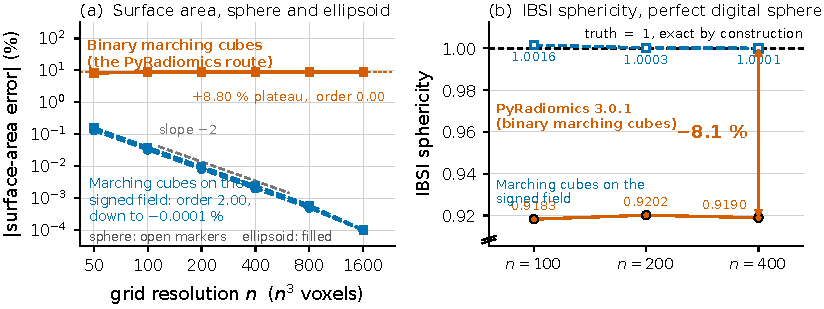
\includegraphics[width=\textwidth]{fig/fig6_surf3d.pdf}
\caption{The same failure in three dimensions. \textbf{(a)} Surface-area error against
resolution: marching cubes on the binary mask plateaus near \pct{+8.8} at observed order $0.00$,
the same algorithm on the signed field falls at order $2$. \textbf{(b)} The consequence for a
shipped feature: sphericity of a \emph{perfect digital sphere} is $1$ by construction, and
PyRadiomics 3.0.1 returns $0.919$ at every resolution we tested.}
\label{fig:surf3d}
\end{figure}


\end{document}
